\ifx\wholebook\relax\else

% --------------------------------------------
% Lulu:

    \documentclass[a4paper,12pt,twoside]{../includes/ThesisStyle}

	\usepackage[T1]{fontenc} %%%key to get copy and paste for the code!
%\usepackage[utf8]{inputenc} %%% to support copy and paste with accents for frnehc stuff
\usepackage{times}
\usepackage{ifthen}
\usepackage{xspace}
\usepackage{alltt}
\usepackage{latexsym}
\usepackage{url}            
\usepackage{amssymb}
\usepackage{amsfonts}
\usepackage{amsmath}
\usepackage{stmaryrd}
\usepackage{enumerate}
\usepackage{cite}
%\usepackage[pdftex,colorlinks=true,pdfstartview=FitV,linkcolor=blue,citecolor=blue,urlcolor=blue]{hyperref}
\usepackage{xspace}
%\usepackage{graphicx}
\usepackage{subfigure}
\usepackage[scaled=0.85]{helvet}
        
        
\newcommand{\sepe}{\mbox{>>}}
\newcommand{\pack}[1]{\emph{#1}}
\newcommand{\ozo}{\textsc{oZone}\xspace}
\newcommand\currentissues{\par\smallskip\textbf{Current Issues -- }}

\newboolean{showcomments}
\setboolean{showcomments}{true}
\ifthenelse{\boolean{showcomments}}
  {\newcommand{\bnote}[2]{
	\fbox{\bfseries\sffamily\scriptsize#1}
    {\sf\small$\blacktriangleright$\textit{#2}$\blacktriangleleft$}
    % \marginpar{\fbox{\bfseries\sffamily#1}}
   }
   \newcommand{\cvsversion}{\emph{\scriptsize$-$Id: macros.tex,v 1.1.1.1 2007/02/28 13:43:36 bergel Exp $-$}}
  }
  {\newcommand{\bnote}[2]{}
   \newcommand{\cvsversion}{}
  } 


\newcommand{\here}{\bnote{***}{CONTINUE HERE}}
\newcommand{\nb}[1]{\bnote{NB}{#1}}
\newcommand{\fix}[1]{\bnote{FIX}{#1}}
%%%% add your own macros 

\newcommand{\sd}[1]{\bnote{Stef}{#1}}
\newcommand{\ja}[1]{\bnote{Jannik}{#1}}
\newcommand{\na}[1]{\bnote{Nico}{#1}}
%%% 


\newcommand{\figref}[1]{Figure~\ref{fig:#1}}
\newcommand{\figlabel}[1]{\label{fig:#1}}
\newcommand{\tabref}[1]{Table~\ref{tab:#1}}
\newcommand{\layout}[1]{#1}
\newcommand{\commented}[1]{}
\newcommand{\secref}[1]{Section \ref{sec:#1}}
\newcommand{\seclabel}[1]{\label{sec:#1}}

%\newcommand{\ct}[1]{\textsf{#1}}
\newcommand{\stCode}[1]{\textsf{#1}}
\newcommand{\stMethod}[1]{\textsf{#1}}
\newcommand{\sep}{\texttt{>>}\xspace}
\newcommand{\stAssoc}{\texttt{->}\xspace}

\newcommand{\stBar}{$\mid$}
\newcommand{\stSelector}{$\gg$}
\newcommand{\ret}{\^{}}
\newcommand{\msup}{$>$}
%\newcommand{\ret}{$\uparrow$\xspace}

\newcommand{\myparagraph}[1]{\noindent\textbf{#1.}}
\newcommand{\eg}{\emph{e.g.,}\xspace}
\newcommand{\ie}{\emph{i.e.,}\xspace}
\newcommand{\ct}[1]{{\textsf{#1}}\xspace}


\newenvironment{code}
    {\begin{alltt}\sffamily}
    {\end{alltt}\normalsize}

\newcommand{\defaultScale}{0.55}
\newcommand{\pic}[3]{
   \begin{figure}[h]
   \begin{center}
   \includegraphics[scale=\defaultScale]{#1}
   \caption{#2}
   \label{#3}
   \end{center}
   \end{figure}
}

\newcommand{\twocolumnpic}[3]{
   \begin{figure*}[!ht]
   \begin{center}
   \includegraphics[scale=\defaultScale]{#1}
   \caption{#2}
   \label{#3}
   \end{center}
   \end{figure*}}

\newcommand{\infe}{$<$}
\newcommand{\supe}{$\rightarrow$\xspace}
\newcommand{\di}{$\gg$\xspace}
\newcommand{\adhoc}{\textit{ad-hoc}\xspace}

\usepackage{url}            
\makeatletter
\def\url@leostyle{%
  \@ifundefined{selectfont}{\def\UrlFont{\sf}}{\def\UrlFont{\small\sffamily}}}
\makeatother
% Now actually use the newly defined style.
\urlstyle{leo}



	\usepackage{amsmath,amssymb}             % AMS Math
% \usepackage[french]{babel}
\usepackage[latin1]{inputenc}
\usepackage[T1]{fontenc}
\usepackage[left=1.5in,right=1.3in,top=1.1in,bottom=1.1in,includefoot,includehead,headheight=13.6pt]{geometry}
\renewcommand{\baselinestretch}{1.05}

\usepackage{multicol}

% Table of contents for each chapter

\usepackage[nottoc, notlof, notlot]{tocbibind}
\usepackage{minitoc}
\setcounter{minitocdepth}{1}
\mtcindent=15pt
% Use \minitoc where to put a table of contents

\usepackage{enumitem}

\usepackage{aecompl}

% Glossary / list of abbreviations

%\usepackage[intoc]{nomencl}
%\renewcommand{\nomname}{List of Abbreviations}
%
%\makenomenclature

% My pdf code

\usepackage[pdftex]{graphicx}
\usepackage[a4paper,pagebackref,hyperindex=true]{hyperref}

\usepackage{pgfplotstable,booktabs,colortbl}
\pgfplotsset{compat=1.8}

% Links in pdf
\usepackage{color}
\definecolor{linkcol}{rgb}{0,0,0.4} 
\definecolor{citecol}{rgb}{0.5,0,0} 

% Change this to change the informations included in the pdf file

% See hyperref documentation for information on those parameters

\hypersetup
{
bookmarksopen=true,
pdftitle="Sista: a Metacircular Architecture for Runtime Optimisation Persistence",
pdfauthor="Clement BERA", 
pdfsubject="Thesis", %subject of the document
%pdftoolbar=false, % toolbar hidden
pdfmenubar=true, %menubar shown
pdfhighlight=/O, %effect of clicking on a link
colorlinks=true, %couleurs sur les liens hypertextes
pdfpagemode=None, %aucun mode de page
pdfpagelayout=SinglePage, %ouverture en simple page
pdffitwindow=true, %pages ouvertes entierement dans toute la fenetre
linkcolor=linkcol, %couleur des liens hypertextes internes
citecolor=citecol, %couleur des liens pour les citations
urlcolor=linkcol %couleur des liens pour les url
}

% definitions.
% -------------------

\setcounter{secnumdepth}{3}
\setcounter{tocdepth}{1}

% Some useful commands and shortcut for maths:  partial derivative and stuff

\newcommand{\pd}[2]{\frac{\partial #1}{\partial #2}}
\def\abs{\operatorname{abs}}
\def\argmax{\operatornamewithlimits{arg\,max}}
\def\argmin{\operatornamewithlimits{arg\,min}}
\def\diag{\operatorname{Diag}}
\newcommand{\eqRef}[1]{(\ref{#1})}

\usepackage{rotating}                    % Sideways of figures & tables
%\usepackage{bibunits}
%\usepackage[sectionbib]{chapterbib}          % Cross-reference package (Natural BiB)
%\usepackage{natbib}                  % Put References at the end of each chapter
                                         % Do not put 'sectionbib' option here.
                                         % Sectionbib option in 'natbib' will do.
\usepackage{fancyhdr}                    % Fancy Header and Footer

% \usepackage{txfonts}                     % Public Times New Roman text & math font
  
%%% Fancy Header %%%%%%%%%%%%%%%%%%%%%%%%%%%%%%%%%%%%%%%%%%%%%%%%%%%%%%%%%%%%%%%%%%
% Fancy Header Style Options

\pagestyle{fancy}                       % Sets fancy header and footer
\fancyfoot{}                            % Delete current footer settings

%\renewcommand{\chaptermark}[1]{         % Lower Case Chapter marker style
%  \markboth{\chaptername\ \thechapter.\ #1}}{}} %

%\renewcommand{\sectionmark}[1]{         % Lower case Section marker style
%  \markright{\thesection.\ #1}}         %

\fancyhead[LE,RO]{\bfseries\thepage}    % Page number (boldface) in left on even
% pages and right on odd pages
\fancyhead[RE]{\bfseries\nouppercase{\leftmark}}      % Chapter in the right on even pages
\fancyhead[LO]{\bfseries\nouppercase{\rightmark}}     % Section in the left on odd pages

\let\headruleORIG\headrule
\renewcommand{\headrule}{\color{black} \headruleORIG}
\renewcommand{\headrulewidth}{1.0pt}
\usepackage{colortbl}
\arrayrulecolor{black}

\fancypagestyle{plain}{
  \fancyhead{}
  \fancyfoot{}
  \renewcommand{\headrulewidth}{0pt}
}

\usepackage{algorithm}
\usepackage[noend]{algorithmic}

%%% Clear Header %%%%%%%%%%%%%%%%%%%%%%%%%%%%%%%%%%%%%%%%%%%%%%%%%%%%%%%%%%%%%%%%%%
% Clear Header Style on the Last Empty Odd pages
\makeatletter

\def\cleardoublepage{\clearpage\if@twoside \ifodd\c@page\else%
  \hbox{}%
  \thispagestyle{empty}%              % Empty header styles
  \newpage%
  \if@twocolumn\hbox{}\newpage\fi\fi\fi}

\makeatother
 
%%%%%%%%%%%%%%%%%%%%%%%%%%%%%%%%%%%%%%%%%%%%%%%%%%%%%%%%%%%%%%%%%%%%%%%%%%%%%%% 
% Prints your review date and 'Draft Version' (From Josullvn, CS, CMU)
\newcommand{\reviewtimetoday}[2]{\special{!userdict begin
    /bop-hook{gsave 20 710 translate 45 rotate 0.8 setgray
      /Times-Roman findfont 12 scalefont setfont 0 0   moveto (#1) show
      0 -12 moveto (#2) show grestore}def end}}
% You can turn on or off this option.
% \reviewtimetoday{\today}{Draft Version}
%%%%%%%%%%%%%%%%%%%%%%%%%%%%%%%%%%%%%%%%%%%%%%%%%%%%%%%%%%%%%%%%%%%%%%%%%%%%%%% 

\newenvironment{maxime}[1]
{
\vspace*{0cm}
\hfill
\begin{minipage}{0.5\textwidth}%
%\rule[0.5ex]{\textwidth}{0.1mm}\\%
\hrulefill $\:$ {\bf #1}\\
%\vspace*{-0.25cm}
\it 
}%
{%

\hrulefill
\vspace*{0.5cm}%
\end{minipage}
}

\let\minitocORIG\minitoc
\renewcommand{\minitoc}{\minitocORIG \vspace{1.5em}}

\usepackage{multirow}
\usepackage{slashbox}

\newenvironment{bulletList}%
{ \begin{list}%
	{$\bullet$}%
	{\setlength{\labelwidth}{25pt}%
	 \setlength{\leftmargin}{30pt}%
	 \setlength{\itemsep}{\parsep}}}%
{ \end{list} }

\newtheorem{definition}{D�finition}
\renewcommand{\epsilon}{\varepsilon}

% centered page environment

\newenvironment{vcenterpage}
{\newpage\vspace*{\fill}\thispagestyle{empty}\renewcommand{\headrulewidth}{0pt}}
{\vspace*{\fill}}



	\graphicspath{{.}{../figures/}}
	\begin{document}
\fi

\chapter{Existing Pharo Runtime}
\label{chap:existing}
\minitoc

%global intro
This chapter describes the Smalltalk dialect Pharo~\cite{Blac09a} and part of its implementation. The Sista architecture was originally designed to improve the performance of the Pharo VM by adding an optimising JIT. Some existing features and implementation details already present in Pharo impacted our design decisions. They are detailed in this chapter to help the reader understanding the design decisions explained in further chapters. The chapter is not meant to explain the whole existing implementation, but only the most relevant points for the thesis. 

Pharo is a pure object-oriented language. Everything is an object, including green threads, classes, method dictionaries or virtual functions. It is dynamically-typed and every call is a virtual call. The virtual machine relies on a virtual function interpreter and a baseline JIT named \emph{Cogit} to gain performance. Pharo directly inherits from Smalltalk-80~\cite{Gold83a} but has additional features such as real closures, exceptions or continuations.

The chapter successively describes some aspects of the Pharo VM, the interface with the language and the Pharo programming language.

%%%%%%%%%%%%%%%%%%%%%%%%%%%%%%%%%%%%%%%%%%%%%%%%%%%%%%%%%%%%%%%%%%%%%%%%%%%%%%%%%%%%%%%%%%%%%%%%%%%%%%%%%%%%%%%%%%%%%%%%%%%%%%

\section{Virtual machine}

The Pharo VM is a flavor of the Cog VM~\cite{Mira08a}. It relies on a v-function interpreter and Cogit, the baseline JIT, to gain performance.

\paragraph{Executable generation.}
Most of the existing VM, inheriting from the original Squeak VM~\cite{Inga97a}, is written in Slang, a subset of Smalltalk. Slang is compiled to C and then to native code through standard C compilers. The execution engine (the memory manager, the interpreter and the baseline JIT) are entirely written in Slang.

In addition to providing some abstractions over machine-specific-details, the slang code has two main advantages over plain C:
\begin{itemize}
	\item \emph{Specifying inlining and code duplication:} To keep the interpreter code efficient, one has to be very careful on what code is inlined in the main interpreter loop and what code is not. In addition, for performance, specific code may need to be duplicated. For example, the interpreter code to push a temporary variable on stack is duplicated 17 times. The 16 first versions are dedicated versions for temporary numbers 0 to 15, the most common cases, and are more efficient because of the use of constants. The 17th version is the generic version, which could be used on any temporary variable but is used in practice for temporary variable 16 and over. Slang allows one to annotate functions to direct Slang to C compilation, by duplicating or inlining specific functions. This way, when a VM developer writes a function, he writes it once and chooses the number of times the function is going to be duplicated or chooses to force the inlining of the function. This feature is very important for uncommon processors where available C compilers are often not as good at optimising C code as on mainstream processors.
	\item \emph{Simulation:} As Slang is a subset of Smalltalk, it can be executed as normal Smalltalk code. This is used to simulate the interpreter and garbage collector behavior. The JIT runtime is simulated using both Slang execution and external processor simulators. Simulation is very convenient to debug the VM as all the Smalltalk debugging tools are available. In addition, the simulator state can be saved and duplicated, which is very convenient to reproduce quickly and many times the same bug happening from a specific runtime state.
\end{itemize}

The executable is generated in two steps as shown on Figure \ref{fig:VMCompilation}, similarly to the RPython toolchain~\cite{Rigo06a}. The first step is to generate the two C files representing the whole execution engine written in Slang using the Slang-to-C compiler. During the second step, a C compiler is called to compile the execution engine and the platform-specific code written directly in C to the executable VM.

\begin{figure}[h!]
    \begin{center}
        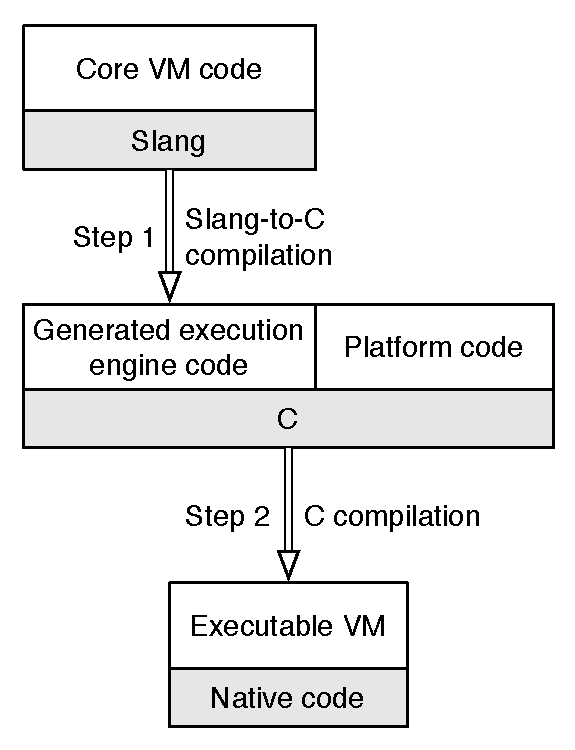
\includegraphics[width=0.45\linewidth]{VMCompilation}
        \caption{VM executable generation}
        \label{fig:VMCompilation}
    \end{center}
\end{figure}

\paragraph{Baseline JIT.}
Cogit is currently used as the baseline JIT. It takes a v-function as input, generates a n-function and installs it. Cogit performs three main kinds of optimisation:
\begin{enumerate}
	\item \emph{Stack-to-register mapping:} As the v-functions are encoded using a stack-based bytecode set, values are constantly pushed and popped off the stack. To avoid this behavior, Cogit simulates the stack state during compilation. When reaching an instruction using values on stack, Cogit uses a dynamic template scheme to generate the native instructions. The simulated stack provides information such as which values are constants or already in registers. Based on this information, Cogit picks one of the available templates for the instruction, uses a linear scan algorithm to allocate registers that do not need to be fixed into specific concrete registers and generates the native instructions.
	\item \emph{Inline caches:} Each virtual call is compiled to an unlinked inline cache. During execution, the inline cache is relinked to a monomorphic, polymorphic or megamorphic inline cache~\cite{Deut84a,Holz91a} when new receiver types are met. The inline caches improve performance but also allows, through n-function introspection, to determine which types were met during previous runs of each virtual call site.
	\item \emph{Calling convention:} Cogit defines specific calling conventions for calls in-between n-functions. Typically, the receiver of the virtual call is always passed by register, and the arguments may or may not be passed by registers depending on how many there are. This is especially efficient to speed-up the inline cache logic and for primitive methods that have an assembly template available as they can directly use the values in registers.
\end{enumerate}

Cogit provides abstractions over the different memory managers supported by the VM (including 32-bits and 64-bits abstractions) and the different assembly back-ends. Most of the optimisations performed are platform-independent, though specific parts, such as inline cache relinking, need to be implemented differently in each back-end. Cogit currently supports four different back-ends in production: x86, x64, ARMv6 and MIPSEL.

\paragraph{Stack frame reification.}
\label{par:frameToContext}
The current VM evolved from the VM specified in the Smalltalk blue book~\cite{Gold83a}. The original specification relied on a spaghetti stack: the execution stack was represented as a linked list of \emph{contexts}, a context being a v-frame in the form of an object. Each context was represented as an object that could, as any other object, be read or written by the program. 

Over the years, Deutsch and Schiffman~\cite{Deut84a} changed the VM internal representation of the stack to improve performance. The new stack representation consists of a linked list of stack pages, where each stack page have stack frames next to each other. Most calls and returns, inside a stack page, can use efficient call and return instructions. Only uncommon calls and returns, across stack pages, need to use slower code. With the current production settings, each stack page has enough size to hold around 50 stack frames and different heuristics are used to make calls and returns across stack pages as uncommon as possible. Figure \ref{fig:StackRepresentation} shows the representation of the stack. In the figure, stack pages hold around 5 stack frames to make it easier to read, but in practice stack pages holding less than 40 frames induce considerable overhead.

\begin{figure}[h!]
    \begin{center}
        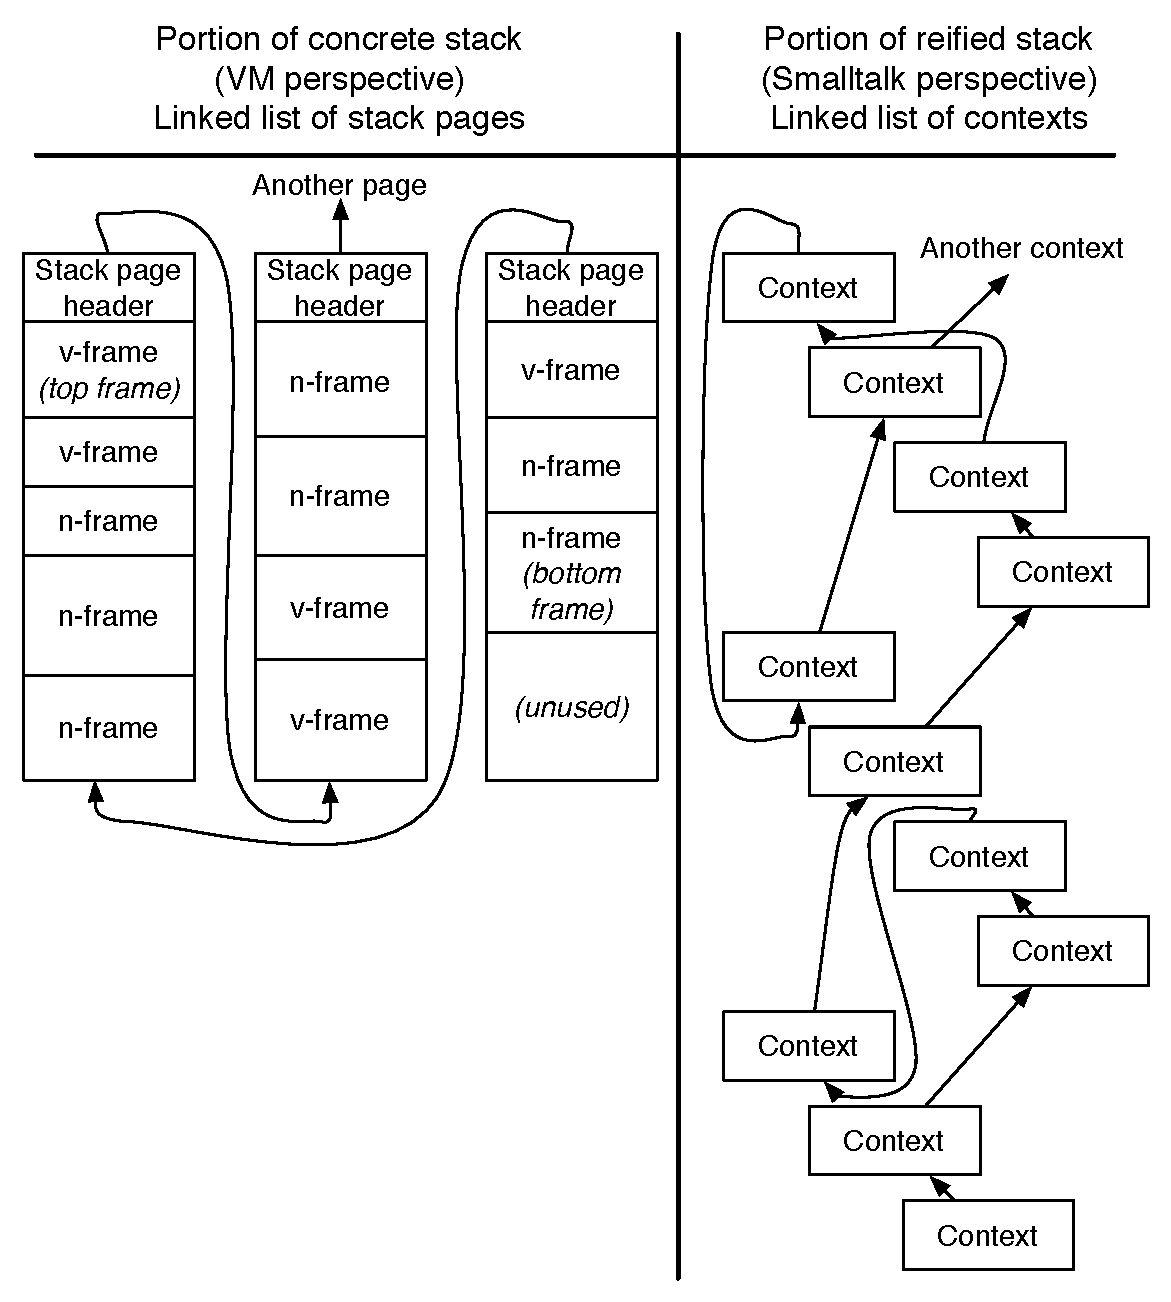
\includegraphics[width=0.52\linewidth]{StackRepresentation}
        \caption{Stack representation}
        \label{fig:StackRepresentation}
    \end{center}
\end{figure}

The VM however still provides the ability for the Smalltalk developer to read and write the reified stack as if it was a linked list of contexts according to the original specification. To do so, the stack is reified as a linked list of contexts on demand. 

The reification of the stack is used in three main places: the debugger, exceptions and continuations. For the latter two, they are implemented in Smalltalk on top of the stack reification, without any special VM support. From Smalltalk, any program can use this feature to instrospect and edit the stack.

Contexts abstract away from low-level details. A context is exactly the same if the VM is started with the interpreter only or with the hybrid interpreter plus baseline JIT runtime. Conceptually, for the Smalltalk developer, the code is interpreted and the contexts always look identical. The VM is responsible to intercept context accesses to read and write concrete v-frames and n-frames.

In this thesis, we suppose that a context is the same thing as a v-frame as the mapping between both has no impact in the design and brings no interesting additional concepts or side-effects. In practice, there are three differences:
\begin{enumerate}
	\item A context is an object while a v-frame uses a low-level representation compliant with the stack.
	\item V-frames have to care about some low-level details, such as calls and returns from v-frames to n-frames and n-frames to v-frames, or the access to the v-function arguments by reading values in the caller frame. 
	\item Contexts have a reference to the caller, as conceptually there is a linked list of contexts, while v-frames are below the caller on stack.
\end{enumerate}
However, both v-frames and contexts use the virtual instruction pointer\footnote{A virtual instruction pointer is a pointer to an instruction in a v-function, by opposition to a native instruction pointer which points to an instruction in a n-function.} and never the native instruction pointer and both refer to the v-function and never to the n-function. Both representations abstract away from machine-specific state as all the values used by the execution are always on stack and never in registers.

To read and write contexts, the VM intercepts all the accesses to the context objects. To do so, contexts can be in two forms. They can be "married" to a v-frame or n-frame, in which case they act as proxies to the frame. The VM then maps reads and writes to read and write the correct field in the frame representation. Alternatively, they can be "single" (for example when instantiated from Smalltalk), which means there is no stack frame on stack representing the context. In this case, the VM can modify the context as a normal object. Upon activation, the VM lazily recreates a v-frame for a single context to execute it (the single context is re-married to a new v-frame). Returns to single contexts are necessarily across stack page boundaries, hence the overhead to test if the caller is a context on heap or a stack frame on stack is required only in the uncommon case of return across stack pages. 

Aggressive stack manipulation (instruction pointer modification, caller modification) may lead the VM to crash. The program performing such operations needs to guarantee it won't happen, this is not the VM responsibility. In addition, these operations require a married context to "divorce" the frame, killing the frame in the process. Upon divorce, the stack page is split in two different stack pages (one part is copied to another memory location). One stack page returns to the single divorced context while the context returns to the other stack page, as shown on Figure \ref{fig:Divorce}. In normal execution the stack is composed exclusively of stack pages, but after stack manipulation from Smalltalk, the stack can be a linked list of stack pages and contexts. 
%as shown on Figure \ref{fig:StackRepresentation2}.

\begin{figure}[h!]
    \begin{center}
        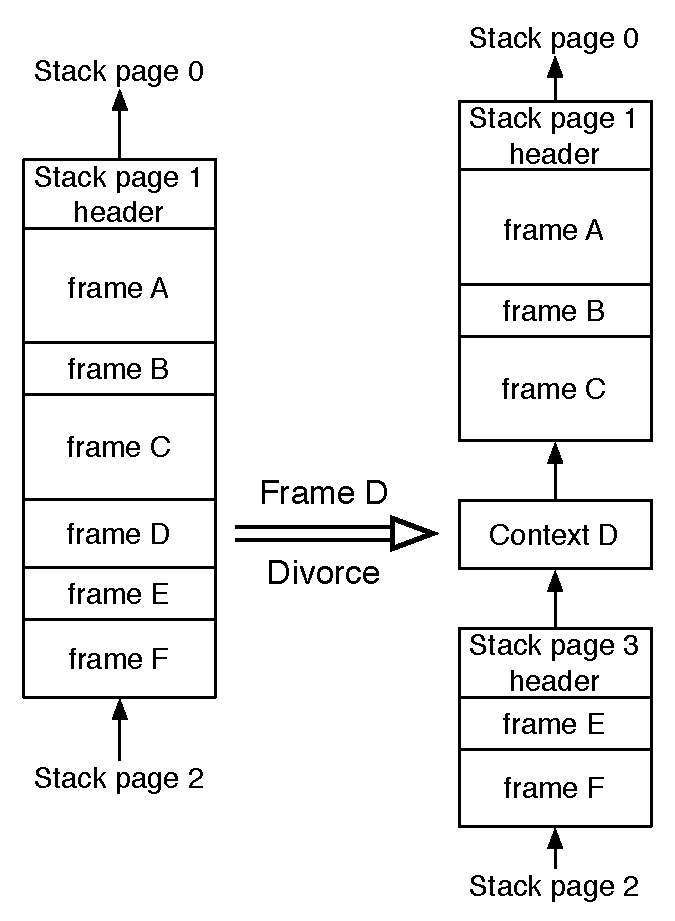
\includegraphics[width=0.55\linewidth]{Divorce}
        \caption{Divorce of stack frame D to context D}
        \label{fig:Divorce}
    \end{center}
\end{figure}

%\begin{figure}[h!]
%    \begin{center}
%        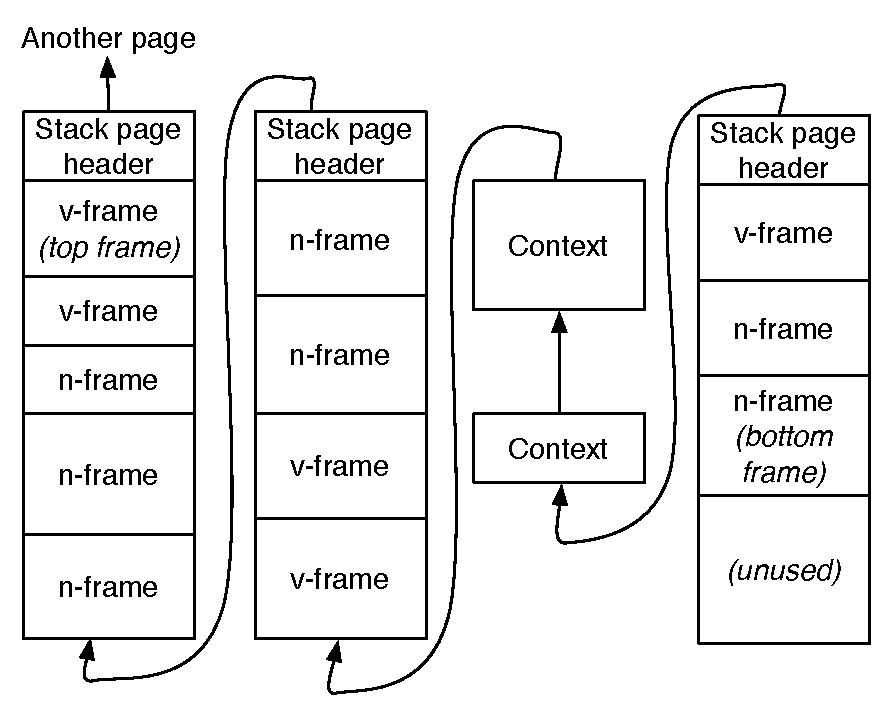
\includegraphics[width=0.7\linewidth]{StackRepresentation2}
%        \caption{Stack representation after stack manipulation}
%        \label{fig:StackRepresentation2}
%    \end{center}
%\end{figure}

Marriages and divorces between stack frames and contexts are not specific to aggressive stack manipulations. They are also used for other features such as snapshots and stack page overflow. In the latter case, as there is a limited number of stack pages (currently 50 in production environments), when a stack page is required and none is available, the VM needs to free a page. To do so, the VM marries then divorces all frames on the least recently used stack page to persist the page in the form of single contexts and re-uses the stack page for the execution of new code. 


%%%%%%%%%%%%%%%%%%%%%%%%%%%%%%%%%%%%%%%%%%%%%%%%%%%%%%%%%%%%%%%%%%%%%%%%%%%%%%%%%%%%%%%%%%%%%%%%%%%%%%%%%%%%%%%%%%%%%%%%%%%%%%%

\section{Language-VM interface}

Pharo interfaces with the VM in two different ways:
\begin{enumerate}
	\item Pharo can instantiate v-functions and install them for execution.
	\item A small list of objects is registered in the VM for direct access.
\end{enumerate}

\paragraph{Virtual function representation.}

As everything is an object in Pharo, virtual functions are objects. A v-function is composed of a function's header, a list of literals, a list of bytecodes and a reference to its source code as shown on Figure \ref{fig:CompiledCode}. The function's header contains information required for the function's execution such as the number of temporary variables or the size of the frame required. The last two literals, in the case of a method, are the selector and the method class, \emph{i.e.,} the class where the method is installed.

\begin{figure}[h!]
    \begin{center}
        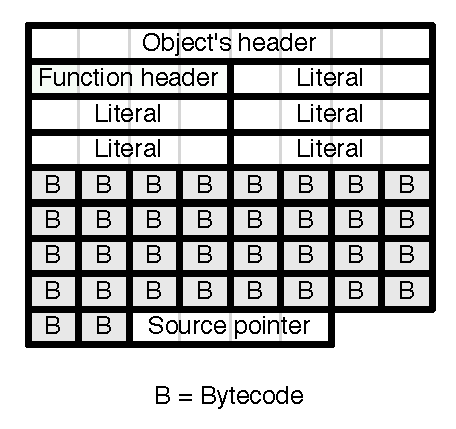
\includegraphics[width=0.38\linewidth]{CompiledCode}
        \caption{Virtual function representation}
        \label{fig:CompiledCode}
    \end{center}
\end{figure}

The bytecode set is stack-based. Most operations are pushing and popping values of the stack. All the operations are untyped and work with any object. One of the main instructions is the virtual call instruction, popping the receiver and arguments from the stack and pushing back the result. The bytecode set also includes conditional and unconditional branches to encode conditions and loops, as well as specific bytecodes to create efficiently closures.


%Move to interface section I believe.

%+ complete list of bytecode instructions, maybe in appendix or a table ? Some of them are duplicated for interpreter performance and compaction (exemple, storePop and push nil), or more or less extended form (uncommon case tke more bytess) but does not really matter.

%Instr - meaning
%In meaning put in emph the variable (index, etc.)

%pushReceiver
%pushLit
%pushThisContext
%pop
%dup
%returnTop
%blockReturnTop

%*2
%pushTemp
%pushInstVar
%pushLitVar
%pushRemoteTemp

%send 
%superSend
%jumpOnTrue
%jumpOnFalse
%jumpForward
%jumpBackward

%createTempVect
%createClosure
%popIntoArray

\subparagraph{Virtual function installation.}

Classes and method dictionaries are normal objects in Pharo. Hence, the installation of a method uses the normal dictionary API, inserting the selector as the key and the method as a value. Method dictionaries, upon modification, request the VM to flush look-up caches for the installed selector. As Pharo is dynamically-typed and through uncommon behavior (stack frame modification, exotic primitives) any method can be called by any object, flushing all the methods matching the selector is easier and safer to implement. Closure's functions are installed inside the method that instantiate them as a literal. %Changing the literal (hence the closure's function) is normally not done in the current runtime.

\subparagraph{Primitive methods.}
\label{par:become}
Virtual methods can be annotated with a primitive number at creation time. A primitive method can be executed through a virtual call, like any other method, but upon activation a low-level function (either a Slang function or the native code generated from an assembly code template, depending on the current state of the runtime) is executed. The low-level code can fail if the receiver and arguments of the primitive method do not meet specific constraints. 

Although primitive methods can be used for performance, most of them provides essential features that could not be implemented otherwise. For example, the addition between two integers is implemented as a primitive, forwarding the operation to the processor's implementation of the addition.

Smalltalk features a set of unconventional primitives, non present in most other programming languages. A notable example is \ct{become:}, a primitive which swaps the references of two objects. If \ct{a become: b}, then all references to \ct{a} now refer to \ct{b}, and all the references to \ct{b} now refer to \ct{a}. This primitive is implemented efficiently based on specific strategies~\cite{Mir15a}.

\paragraph{Registered objects.}
\label{par:regObjects}
 An array of registered objects\footnote{Smalltalk developers use the term special object array for this array} is accessible both to the Pharo VM and from the language. This array contains multiple objects that need to be accessed directly by the VM, for example the objects \ct{nil, true} and \ct{false}. Any new object can be registered in the array and the array can grow on demand.

Among registered objects are specific selectors, such as the \ct{\#doesNotUnderstand:} selector. When a look-up performed by the VM does not find any method to activate (the selector is not implemented for the given receiver), the VM instead performs a virtual call, using the same receiver, the registered \ct{\#doesNotUnderstand:} selector and reifies the virtual call as an object (which class is also registered) containing the original selector, the arguments and the look-up class in case of a super send. 

The registered objects allows some flexibility in the VM: each entry can be modified from the language, changing the VM behavior, without recompiling the VM.

%%%%%%%%%%%%%%%%%%%%%%%%%%%%%%%%%%%%%%%%%%%%%%%%%%%%%%%%%%%%%%%%%%%%%%%%%%%%%%%%%%%%%%%%%%%%%%%%%%%%%%%%%%%%%%%%%%%%%%%%%%%%%%%

\section{Language relevant features}

This section details two main aspects of the programming language: native thread management and snapshots.

\paragraph{Native thread management.}

Pharo features a global interpreter lock, similarly to Python. Only calls to external libraries through the foreign function interface and specific virtual machine extensions have access to the other native threads. Smalltalk execution, including bytecode interpretation, machine code execution, just-in-time compilation and garbage collection are not done concurrently. Being single-threaded has a impact on design decisions because several other VMs implement the optimising JIT in concurrent native threads to the application~\cite{Arn00}.

%TODO, closures and NLR?

\paragraph{Snapshots.}
\label{par:snapshot}

In the context of Smalltalk, a snapshot\footnote{Smalltalk developers use the term \emph{image} instead of snapshot.} is a sequence of bytes that represents a serialized form of all the objects present at a precise moment in the runtime. As everything is an object in Smalltalk, including green threads, classes and v-functions, the virtual machine starts-up by loading all the objects from a snapshot and resumes the execution based on the green thread that was active at snapshot time. In fact, this is the normal way of launching a Smalltalk runtime. 

One interesting problem in snapshots is how to save the execution stack, \ie the green threads. To perform a snapshot, each stack frame is reified into a context and only objects are saved in the snapshot. When the snapshot is restarted, the VM recreates a stack frame for each context lazily. 

In any case, snapshots are platform-independent so they cannot save n-frames. In the Pharo VM for example, a snapshot can be taken on a laptop using a x86 processor and restarted on a raspberry pi using a ARMv6 processor.

%%%%%%%%%%%%%%%%%%%%%%%%%%%%%%%%%%%%%%%%%%%%%%%%%%%%%%%%%%%%%%%%%%%%%%%%%%%%%%%%%%%%%%%%%%%%%%%%%%%%%%%%%%%%%%%%%%%%%%%%%%%%%%%

%Maybe conclusion summary in 1 sentence of chapter + what comes next
\section*{Conclusion} 

The chapter described the aspects and features of Pharo relevant for the thesis. The following chapter describes the overall architecture discussed in the thesis.

\ifx\wholebook\relax\else
    \end{document}
\fi